\subsection{User interface}\label{subsec:user-interface}

The main purpose of the user interface is to load the pump.
I.e., the pump and the connected tube, when not used previously, do not carry any acid.
If the pump cycle would activate, nothing would be distributed until the formic acid reached the end of the tube.
A UI is therefore needed, to manually load the pump and the tube before the operation can start autonomously.

The UI is implemented with an Android application containing two simple screens.
The first screen, scans for bluetooth devices so a bee-keeper can find and connect to the processor.
When the connection is established, a second screen is opened.
This screen contains a card, showing the last measured temperature and a button to start or stop the pump, depending on its current state.

\begin{figure}[h]
    \centering
    \begin{minipage}{0.5\textwidth}
        \centering
        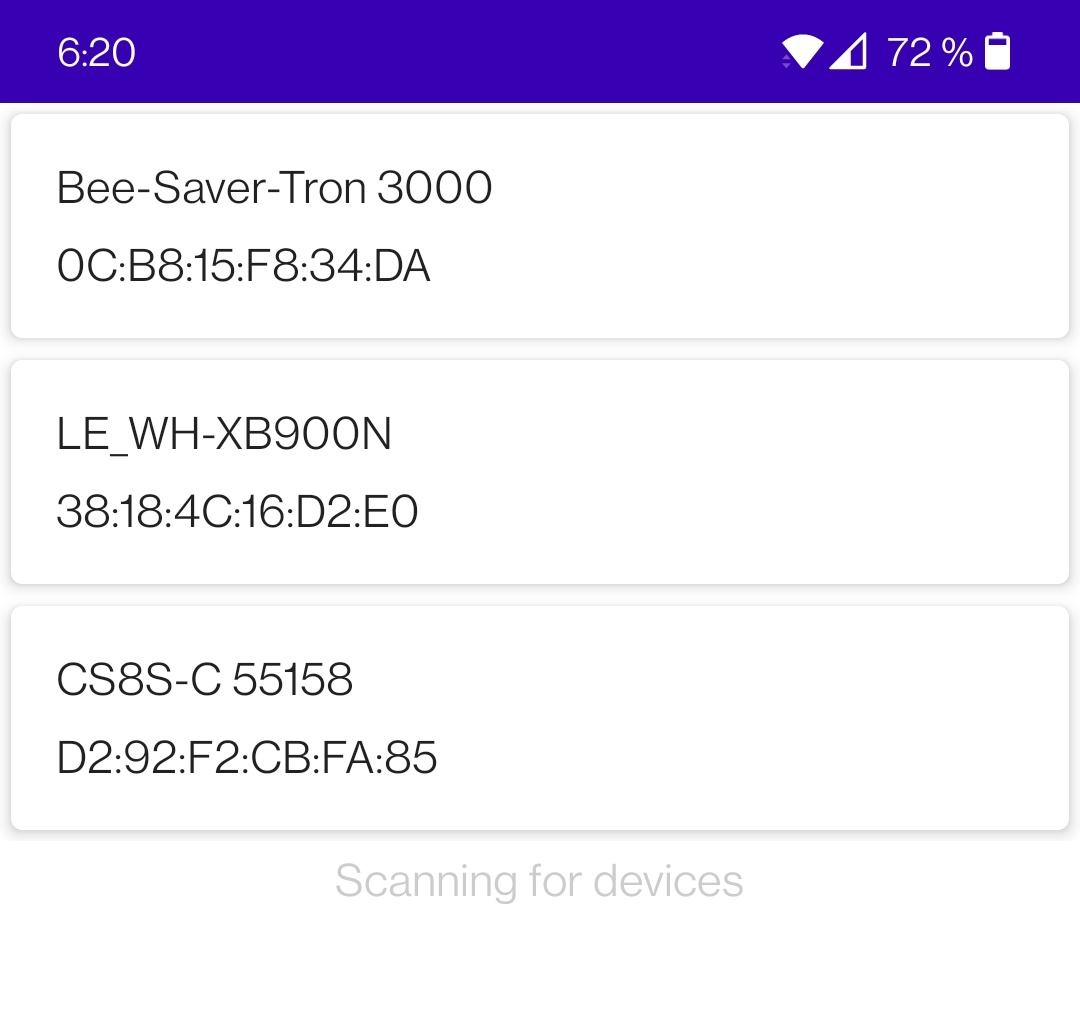
\includegraphics[width=0.9\textwidth]{img/bluetooth-list}
        \caption{List of found bluetooth devices}
        \label{fig:bluetooth-devices}
    \end{minipage}\hfill
    \begin{minipage}{0.5\textwidth}
        \centering
        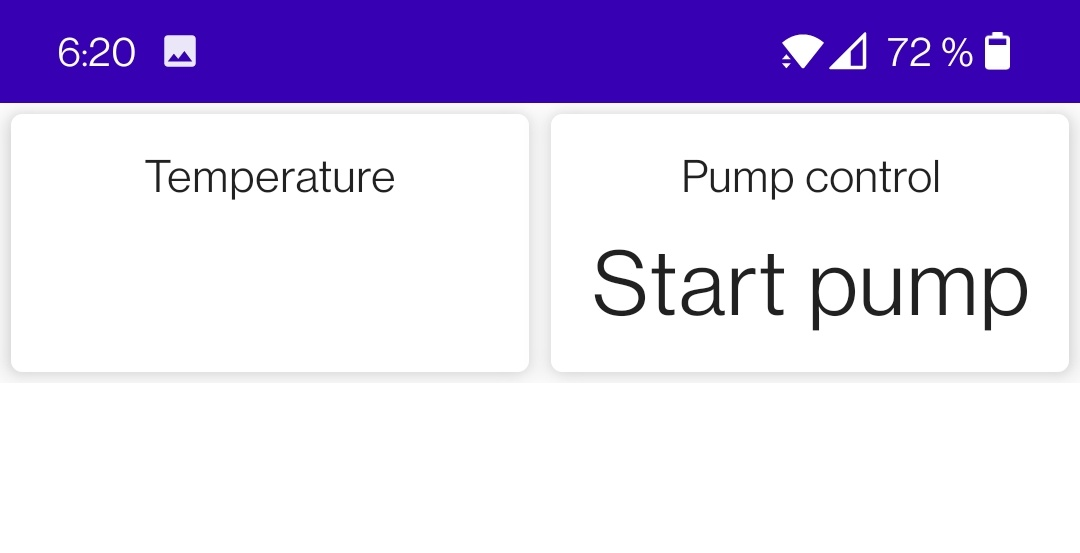
\includegraphics[width=0.9\textwidth]{img/control}
        \caption{Control screen}
        \label{fig:control-screen}
    \end{minipage}
\end{figure}

Figure \ref{fig:bluetooth-devices} shows the first screen displaying found bluetooth devices.
The entry called ''Bee-Saver-Tron 3000'' is the currently set name of the processor.
Clicking on this entry establishes a connection and the second screen, shown in Figure \ref{fig:control-screen}, is opened.
On the left, the temperature is normally displayed.
It is not in this case, as the connection has been made with a test processor, not connected to an actual sensor.
On the right, the button to issue the start command is shown.

